%\thispagestyle{empty}
\section{Introduction}
\label{introductions}

The CMS tracker material is not negligible as a consequence of the
massive mechanical structure and the amount of services needed to
support and run such a large, complex and highly granular tracking device.

As a consequence of that, the effect of the interactions of particles
with the material are not negligible. 


A robust method for the Material Budget estimation, exploited by many
past experiments, is based on photon conversions. The idea is that the
material radiography, provided by the position of reconstructed photon
conversion vertices, allows for the visualisation of detector layers
and service structures and that the conversions rate, if properly
accounted, provides an estimate of the amount of material in the
detector volume.

At the LHC many photons are produced from $\pi^0$ decays in minimum bias events; 
as shown in Figure~\ref{ptMC}, the $p_T$ spectrum of such photons is
very soft and the electron and positron produced in the conversion 
do not have enough transverse momentum to reach the CMS electromagnetic calorimeter.
Therefore, conversions need to be reconstructed with a tracker standalone algorithm.

\begin{figure}[!hbtp]
\centering
%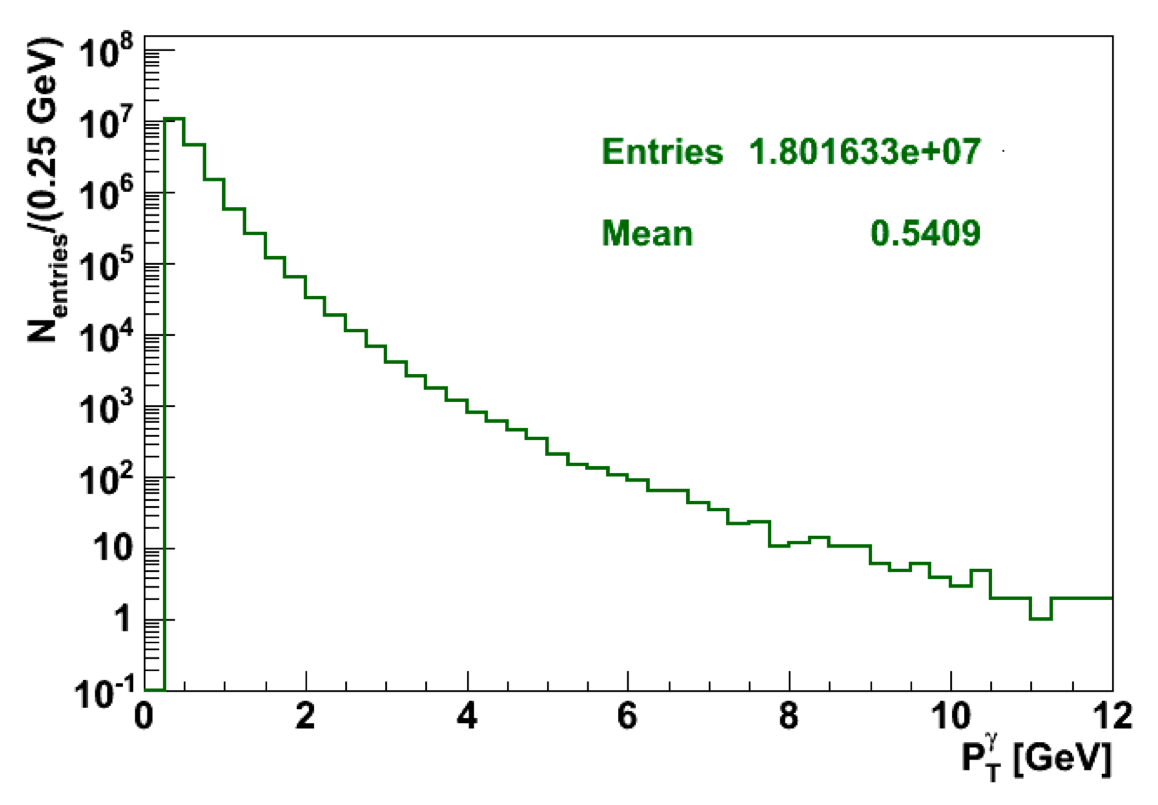
\includegraphics[width=.45\textwidth]{ptMC.png}
\caption{Transverse momentum spectrum of converted photons in minimum
  bias MC events at $\sqrt{s}=900\GeV$.}
\label{ptMC}
\end{figure}

The present analysis makes use of the algorithm described in~\cite{nancy}.
It allows the reconstruction of low-$p_T$ photons ($\geq 0.4\GeV$)
without any request of ECAL match. The main signature for the
conversion identification is the reconstruction of two opposite
charged tracks with tangent direction at the point where they form a
detached vertex. The vertex fit is performed with the \emph{Kinematic
  Constraint Vertex Fitter}.



